\documentclass[aspectratio=169]{beamer}
\usetheme[block=fill]{metropolis}
\usepackage{tikz}
\usetikzlibrary{shapes.geometric, arrows.meta, positioning, calc}

\title{Building a Reproducible Scholarly Search Toolkit}
\subtitle{Episode 22: The Harness Tutorial Conclusion}
\author{Scholar Search Kit}
\date{}

\begin{document}

\begin{frame}[plain]
  \titlepage
\end{frame}

\begin{frame}{Episode Goal}
  \begin{alertblock}{The Goal}
    Summarize what we built, reiterate the importance of Clean Architecture in research, and hand over the keys to the community.
  \end{alertblock}
  \vspace{0.5cm}
  We started with a mess of API scripts. We ended with an enterprise-grade, extensible, reproducible search tool.
\end{frame}

\begin{frame}{The Final Architecture}
  \begin{center}
  \resizebox{0.8\linewidth}{!}{
  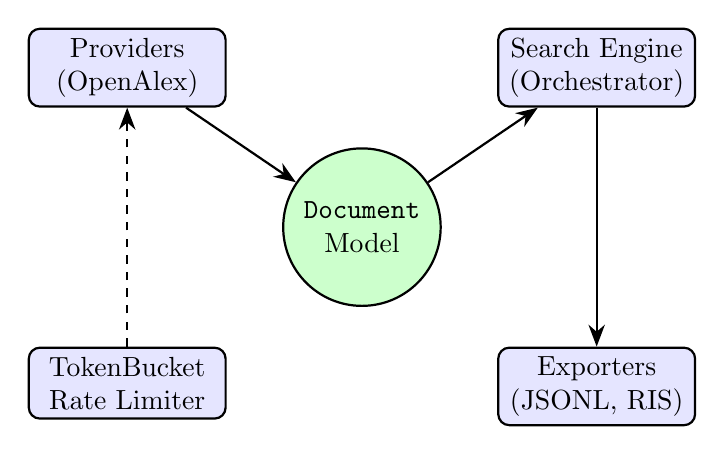
\begin{tikzpicture}[
      node distance=0.8cm and 1cm,
      comp/.style={rectangle, draw, thick, rounded corners, minimum width=2.5cm, align=center, fill=blue!10},
      core/.style={circle, draw, thick, minimum size=2cm, align=center, fill=green!20},
      arrow/.style={-{Stealth[scale=1.2]}, thick}
    ]
    
    \node[core] (doc) {\texttt{Document}\\Model};
    
    \node[comp, above left=of doc] (prov) {Providers\\(OpenAlex)};
    \node[comp, below left=of doc] (rate) {TokenBucket\\Rate Limiter};
    \node[comp, above right=of doc] (eng) {Search Engine\\(Orchestrator)};
    \node[comp, below right=of doc] (exp) {Exporters\\(JSONL, RIS)};
    
    \draw[arrow] (prov) -- (doc);
    \draw[arrow, dashed] (rate) -- (prov);
    \draw[arrow] (doc) -- (eng);
    \draw[arrow] (eng) -- (exp);
  \end{tikzpicture}
  }
  \end{center}
\end{frame}

\begin{frame}{Key Takeaways}
  \begin{block}{Why We Built This}
    \begin{itemize}
        \item \textbf{Decoupling:} Business logic doesn't care about HTTP status codes.
        \item \textbf{Reproducibility:} Every output is mathematically proven and receipted.
        \item \textbf{Resilience:} The network \textit{will} fail; the code must survive.
    \end{itemize}
  \end{block}
\end{frame}

\begin{frame}{What's Next?}
  \begin{alertblock}{The Future}
    This is v0.1.0. It's just the beginning.
  \end{alertblock}
  
  \begin{itemize}
      \item Adding Semantic Scholar and PubMed providers.
      \item Parallel multi-provider asynchronous querying.
      \item A web dashboard for visual deduplication.
  \end{itemize}
  \vspace{0.5cm}
  \textbf{Thank you for watching the series!}
\end{frame}

\end{document}
